\chapter{Экспериментальный раздел}
\label{sec:experiment}

В данном разделе описаны проведенные эксперименты, призванные определить
точность разработанной системы при аутентификации пользователей, а также
определить необходимые для работы системы параметры.

\section{Планирование эксперимента}

\subsection{Определение точности системы аутентификации}

При анализе биометрических систем, точность системы
определяется вероятностями совершения ошибок I-ого и II-ого рода:

\begin{enumerate}
\item Аутентификация завершилась неудачно для аутентичного источника речи (ложный отказ);
\item Аутентификация прошла успешно, но источник речи в действительности не аутентичен зарегистрированному (несанкционированный вход).
\end{enumerate}

Требуемый баланс между этими показателями достигается путем варьирования
значения порога вхождения. Частота ошибок (\important{Equal Error Rate}) --
значение вероятности при таком пороге вхождения, когда вероятности ошибок I-ого
и II-ого рода равны.

Для более подробного отражения качественных характеристик системы используются
так называемые DET-кривые (Detection Error Trade-off curves)~\cite{Alvin97DET}. На оси $x$
DET-кривой отражается процент ложного отказа, при этом на оси $y$ отражается
процент ложного положительного решения (при одинаковом пороге). Варьируя
значение порога вхождения, получаем кривую. Данный метод позволяет качественно и
количественно сравнивать
показатели системы при изменении параметров.

\subsection{Описание экспериментов}

Для работы системы необходимо определить значения ряда параметров, в частности:

\begin{itemize}

\item Количество фраз для стадии обучения модели (см.
раздел~\ref{sec:construct:enrollment}). При создании персональной модели
источника речи, пользователю необходимо произнести ключевую фразу несколько раз,
чтобы накопить достаточное для обучения модели количество речевых данных.
Эксперимент позволит определить такое минимальное количество, при котором для
тестируемой выборки будут соблюдены требования, предъявляемые к точности
аутентификации;

\item Величина порога вхождения (реализованный алгоритм голосовой верификации даёт
численную оценку правдоподобия проверяемой гипотезы, но для принятия решения
необходимо определить, достаточна ли полученная величина для того, чтобы с
уверенностью говорить о положительном результате аутентификации). От данной
величины напрямую зависит чувствительность системы, поэтому, если она выбирается
глобально, необходимо получить её экспериментально, то есть найти минимальное
значение, при котором исключаются ошибки второго рода (ложные срабатывания).

\item Влияние применения алгоритма удаления тишины на точность аутентификации (алгоритм
рассмотрен в разделе~\ref{sec:construct:silence_remove}). Целью эксперимента
является определение параметров алгоритма, при которых достигается наибольшая
точность (в рамках имеющейся тестовой выборки).

\item Количество компонент смеси гауссиан. Применяемый метод для моделирования
источника речи параметризуется количеством компонент смеси. Чем больше это
количество, тем, теоретически, точнее ожидаемая точность аутентификации.
Эксперимент позволит определить минимальное количество, при котором
удовлетворяются требования точности.

\item Анализ качества системы при использовании различных методов обучения. В
рамках проекта реализовано два различных подхода к обучению модели: алгоритм
Expectation-Maximization и адаптивное обучение с помощью алгоритма MAP (Max a
posteriori adaptation). Эксперимент позволит сравнить два метода обучения.

\end{itemize}

\subsection{Описание входных данных}

Для проведения экспериментов была составлена выборка, состоящая из 30 человек,
из них 16 мужчин и 15 женщин. Каждый человек записывал одну и ту же фразу, что
позволяет анализировать способность системы различать особенности речи отдельных
людей. Запись проходила в обстановке, максимально приближенной к условиям
эксплуатации программного комплекса: каждый источник речи использовал для записи
собственный микрофон и записывался в домашних условиях, удаленно. Средняя длина
записанной фразы: $2.913$ секунд. Количество записей в расчете на человека:
$60$.

\subsubsection*{Сбор данных}

Для сбора данных в систему был включен модуль, использующий
разработанную базу для записи и отправки голосовых данных от анонимных
пользователей и сохранения их в файловой системе с кратким описанием, что
позволило автоматизировать последующую обработку. Запись данных при этом
происходила удаленно. Форма для записи и отправки голосовых данных представлена
на рисунке~\ref{fig:ui:voice_upload}. Процесс записи аналогичен процессу
создания персональной голосовой модели, описанному в
разделе~\ref{sec:manual:enrollment}. После записи, участнику тестирования
необходимо было заполнить форму с описанием сессии, которая сохранялась в базе
данных для последующей обработки в процессе эксперимента.

\begin{figure}[ht!]
\center{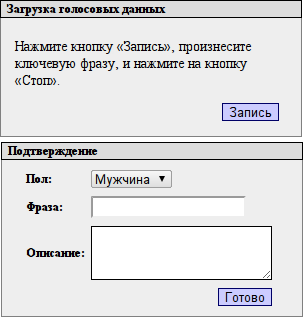
\includegraphics[width=72mm]{static_include/voice_upload.png}}
\caption{Диалог записи и загрузки голосовых данных}
\label{fig:ui:voice_upload}
\end{figure}

\section{Анализ результатов}



